\refstepcounter{chapter}
\chapter*{Appendix B}
\addcontentsline{toc}{chapter}{Appendix B}
\markboth{Appendix B}{Appendix B}
\label{app:lidar}

\begin{table}[H]
\centering
\setlength{\tabcolsep}{1.6pt}
\resizebox{\textwidth}{!}{%
\begin{tabular}{lccccc|ccccccccc}
\toprule
 & \multicolumn{5}{c|}{Rear, $|x_{\mathrm{rel}}|$ [m]} & \multicolumn{9}{c}{Front, $x_{\mathrm{rel}}$ [m]} \\
Session & 60--50 & 50--40 & 40--30 & 30--20 & 20--10 & 10--20 & 20--30 & 30--40 & 40--50 & 50--60 & 60--70 & 70--80 & 80--90 & 90--100 \\
\midrule
07/26\_TUM & -- & 0.67 & 0.42 & 0.20 & 0.08 & 0.05 & 0.19 & 0.09 & 0.11 & 0.17 & 0.18 & 0.21 & 0.23 & 0.25 \\
08/03\_Kinetiz & 0.38 & 0.30 & 0.32 & 0.15 & 0.16 & 0.18 & 0.16 & 0.15 & 0.15 & 0.15 & 0.20 & 0.21 & 0.24 & 0.21 \\
10/12 (EVA+LIVIA) & -- & 0.28 & 0.22 & 0.09 & 0.04 & 0.04 & 0.04 & 0.17 & 0.06 & 0.07 & 0.09 & 0.08 & 0.08 & 0.16 \\
10/13 (EVA+LIVIA) & 0.23 & 0.24 & -- & -- & -- & -- & -- & 0.17 & 0.17 & 0.10 & 0.07 & 0.11 & 0.21 & 0.19 \\
10/14\_eva & -- & 0.15 & 0.12 & 0.14 & 0.53$^{*}$ & 0.10 & 0.08 & 0.08 & 0.10 & 0.10 & 0.12 & 0.16 & 0.15 & 0.13 \\
10/14-02 (EVA+LIVIA) & -- & 0.38 & 0.21 & 0.12 & 0.07 & 0.08 & 0.08 & 0.11 & 0.12 & 0.08 & 0.12 & 0.13 & -- & -- \\
10/14-04 (EVA) & -- & -- & 0.17 & 0.10 & 0.08 & 0.08 & 0.14 & 0.15 & 0.19 & 0.14 & 0.13 & 0.13 & 0.11 & 0.10 \\
10/16 (EVA+LIVIA) & -- & -- & 0.29 & 0.18 & 0.20 & 0.06 & 0.07 & 0.10 & 0.10 & 0.09 & 0.11 & 0.14 & 0.15 & 0.10 \\
\bottomrule
\end{tabular}}
\par\vspace{2pt}{\footnotesize $^{*}$ 10/14\_eva: at 10--20\,m behind the opponent is almost on the ego axis (median $|y_{\mathrm{rel}}|\approx2$\,m, rear blind strip); without the samples with $|y_{\mathrm{rel}}|<2$\,m: $\sigma_x=0.12$\,m, $\sigma_y=0.18$\,m.}
\caption{LiDAR Clustering: standard deviation of the longitudinal error $\sigma_x$ [m] vs $x_{\mathrm{rel}}$ (10\,m bins).}
\label{tab:clust_sx}
\end{table}

\begin{table}[H]
\centering
\setlength{\tabcolsep}{1.6pt}
\resizebox{\textwidth}{!}{%
\begin{tabular}{lccccc|ccccccccc}
\toprule
 & \multicolumn{5}{c|}{Rear, $|x_{\mathrm{rel}}|$ [m]} & \multicolumn{9}{c}{Front, $x_{\mathrm{rel}}$ [m]} \\
Session & 60--50 & 50--40 & 40--30 & 30--20 & 20--10 & 10--20 & 20--30 & 30--40 & 40--50 & 50--60 & 60--70 & 70--80 & 80--90 & 90--100 \\
\midrule
07/26\_TUM & -- & 0.69 & 0.35 & 0.19 & 0.08 & 0.09 & 0.25 & 0.13 & 0.16 & 0.23 & 0.27 & 0.27 & 0.30 & 0.43 \\
08/03\_Kinetiz & 0.49 & 0.39 & 0.33 & 0.29 & 0.21 & 0.08 & 0.10 & 0.09 & 0.10 & 0.14 & 0.14 & 0.35 & 0.38 & 0.39 \\
10/12 (EVA+LIVIA) & -- & 0.33 & 0.20 & 0.11 & 0.08 & 0.05 & 0.06 & 0.09 & 0.11 & 0.15 & 0.19 & 0.23 & 0.31 & 0.54 \\
10/13 (EVA+LIVIA) & 0.51 & 0.44 & -- & -- & -- & -- & -- & 0.07 & 0.16 & 0.18 & 0.16 & 0.28 & 0.31 & 0.37 \\
10/14\_eva & -- & 0.17 & 0.18 & 0.31 & 0.47$^{*}$ & 0.10 & 0.11 & 0.09 & 0.13 & 0.13 & 0.19 & 0.25 & 0.21 & 0.28 \\
10/14-02 (EVA+LIVIA) & -- & 0.63 & 0.43 & 0.14 & 0.07 & 0.08 & 0.09 & 0.14 & 0.17 & 0.16 & 0.19 & 0.23 & -- & -- \\
10/14-04 (EVA) & -- & -- & 0.38 & 0.23 & 0.10 & 0.05 & 0.13 & 0.20 & 0.11 & 0.17 & 0.26 & 0.25 & 0.23 & 0.29 \\
10/16 (EVA+LIVIA) & -- & -- & 0.44 & 0.29 & 0.29 & 0.12 & 0.08 & 0.20 & 0.11 & 0.14 & 0.23 & 0.25 & 0.19 & 0.23 \\
\bottomrule
\end{tabular}}
\par\vspace{2pt}{\footnotesize $^{*}$ 10/14\_eva: at 10--20\,m behind the opponent is almost on the ego axis (median $|y_{\mathrm{rel}}|\approx2$\,m, rear blind strip); without the samples with $|y_{\mathrm{rel}}|<2$\,m: $\sigma_x=0.12$\,m, $\sigma_y=0.18$\,m.}
\caption{LiDAR Clustering: standard deviation of the lateral error $\sigma_y$ [m] vs $x_{\mathrm{rel}}$ (10\,m bins).}
\label{tab:clust_sy}
\end{table}

\begin{table}[H]
\centering
\setlength{\tabcolsep}{1.6pt}
\resizebox{\textwidth}{!}{%
\begin{tabular}{lccccc|ccccccccc}
\toprule
 & \multicolumn{5}{c|}{Rear, $|x_{\mathrm{rel}}|$ [m]} & \multicolumn{9}{c}{Front, $x_{\mathrm{rel}}$ [m]} \\
Session & 60--50 & 50--40 & 40--30 & 30--20 & 20--10 & 10--20 & 20--30 & 30--40 & 40--50 & 50--60 & 60--70 & 70--80 & 80--90 & 90--100 \\
\midrule
07/26\_TUM & -- & $+0.28$ & $+0.24$ & $+0.26$ & $+0.15$ & $+0.01$ & $0.00$ & $-0.01$ & $-0.04$ & $-0.08$ & $-0.09$ & $-0.08$ & $-0.13$ & $-0.19$ \\
08/03\_Kinetiz & $+0.30$ & $+0.29$ & $+0.27$ & $+0.24$ & $+0.13$ & $-0.01$ & $-0.01$ & $-0.03$ & $-0.14$ & $-0.16$ & $-0.20$ & $-0.29$ & $-0.28$ & $-0.23$ \\
10/12 (EVA+LIVIA) & -- & $+0.37$ & $+0.36$ & $+0.30$ & $+0.23$ & $+0.09$ & $+0.07$ & $+0.01$ & $+0.01$ & $-0.02$ & $-0.02$ & $0.00$ & $-0.05$ & $-0.06$ \\
10/13 (EVA+LIVIA) & $+0.30$ & -- & -- & -- & -- & -- & -- & $0.00$ & $+0.04$ & $-0.01$ & $0.00$ & $-0.03$ & $-0.08$ & $-0.11$ \\
10/14\_eva & $+0.34$ & $+0.36$ & $+0.30$ & $+0.26$ & $+0.24$ & $+0.04$ & $+0.02$ & $0.00$ & $+0.01$ & $-0.01$ & $-0.01$ & $-0.05$ & $-0.09$ & $-0.10$ \\
10/14-02 (EVA+LIVIA) & $+0.47$ & $+0.43$ & $+0.39$ & $+0.37$ & $+0.23$ & $+0.14$ & $+0.06$ & $0.00$ & $-0.01$ & $-0.03$ & $+0.09$ & $+0.08$ & $+0.05$ & -- \\
10/14-04 (EVA) & -- & -- & $+0.30$ & $+0.29$ & $+0.24$ & $+0.08$ & $+0.03$ & $+0.03$ & $0.00$ & $-0.04$ & $-0.04$ & $-0.01$ & $-0.07$ & $-0.10$ \\
10/16 (EVA+LIVIA) & $+0.43$ & $+0.40$ & $+0.37$ & $+0.33$ & $+0.28$ & $+0.04$ & $0.00$ & $+0.04$ & $-0.05$ & $-0.04$ & $-0.06$ & $-0.07$ & $-0.14$ & $-0.23$ \\
\bottomrule
\end{tabular}}
\caption{LiDAR PointPillars: mean longitudinal error $e_x$ [m] vs $x_{\mathrm{rel}}$ (10\,m bins). Reference offset removed.}
\label{tab:pp_ex}
\end{table}

\begin{table}[H]
\centering
\setlength{\tabcolsep}{4pt}\small
\begin{tabular}{lccccccccc}
\toprule
Session & \multicolumn{9}{c}{$|x_{\mathrm{rel}}|$ [m]} \\
\cmidrule(l){2-10}
 & 10--20 & 20--30 & 30--40 & 40--50 & 50--60 & 60--70 & 70--80 & 80--90 & 90--100 \\
\midrule
\multicolumn{10}{l}{\textit{Rear ($x_{\mathrm{rel}}<0$)}} \\
07/26\_TUM & 0.42 & 0.57 & 0.64 & 0.75 & 0.90 & 0.69 & 0.91 & 0.92 & 1.12 \\
08/03\_Kinetiz & 0.43 & 0.52 & 0.57 & 0.66 & 0.68 & 0.62 & 0.83 & 0.94 & 0.83 \\
10/12 (EVA+LIVIA) & 0.41 & 0.56 & 0.60 & 0.62 & 0.74 & 0.75 & 0.77 & 0.95 & 0.75 \\
10/13 (EVA+LIVIA) & -- & -- & 0.48 & 0.65 & 0.88 & 0.74 & 0.63 & 0.85 & 1.00 \\
10/14\_eva & 0.43 & 0.50 & 0.62 & 0.65 & 0.61 & 0.63 & 0.49 & -- & -- \\
10/14-02 (EVA+LIVIA) & 0.62 & 0.58 & 0.61 & 0.63 & 0.66 & 0.70 & 0.60 & 0.61 & 0.80 \\
10/14-04 (EVA) & 0.46 & 0.57 & 0.64 & 0.60 & 0.76 & -- & -- & -- & -- \\
10/16 (EVA+LIVIA) & 0.47 & 0.51 & 0.70 & 0.73 & 0.84 & 0.88 & 0.90 & 1.04 & 0.91 \\
\midrule
\multicolumn{10}{l}{\textit{Front ($x_{\mathrm{rel}}>0$)}} \\
07/26\_TUM & 0.45 & 0.45 & 0.52 & 0.57 & 0.63 & 0.65 & 0.62 & 0.77 & 0.71 \\
08/03\_Kinetiz & 0.52 & 0.53 & 0.53 & 0.53 & 0.54 & 0.59 & 0.68 & 0.82 & 0.82 \\
10/12 (EVA+LIVIA) & 0.39 & 0.51 & 0.54 & 0.62 & 0.63 & 0.68 & 0.69 & 0.80 & 0.76 \\
10/13 (EVA+LIVIA) & -- & -- & -- & 0.57 & 0.62 & 0.72 & 0.64 & 0.79 & 0.67 \\
10/14\_eva & 0.35 & 0.45 & 0.49 & 0.54 & 0.59 & 0.67 & 0.74 & 0.93 & 0.91 \\
10/14-02 (EVA+LIVIA) & 0.46 & 0.50 & 0.48 & 0.56 & 0.49 & 0.53 & 0.55 & 0.79 & 0.71 \\
10/14-04 (EVA) & -- & 0.32 & 0.42 & 0.53 & 0.52 & 0.48 & 0.48 & 0.73 & 0.66 \\
10/16 (EVA+LIVIA) & 0.69 & 0.57 & 0.53 & 0.63 & 0.75 & 0.83 & 0.91 & 0.86 & 0.63 \\
\bottomrule
\end{tabular}
\caption{RaDAR: standard deviation of the longitudinal error $\sigma_x$ [m] vs $|x_{\mathrm{rel}}|$ (10\,m bins).}
\label{tab:rad_sx}
\end{table}

\begin{table}[H]
\centering
\setlength{\tabcolsep}{4pt}\small
\begin{tabular}{lccccccccc}
\toprule
Session & \multicolumn{9}{c}{$|x_{\mathrm{rel}}|$ [m]} \\
\cmidrule(l){2-10}
 & 10--20 & 20--30 & 30--40 & 40--50 & 50--60 & 60--70 & 70--80 & 80--90 & 90--100 \\
\midrule
\multicolumn{10}{l}{\textit{Rear ($x_{\mathrm{rel}}<0$)}} \\
07/26\_TUM & $+0.31$ & $+0.06$ & $-0.16$ & $-0.16$ & $-0.17$ & $+0.17$ & $-0.16$ & $-0.05$ & $-0.11$ \\
08/03\_Kinetiz & $+0.56$ & $+0.10$ & $+0.22$ & $+0.05$ & $+0.19$ & $+0.20$ & $+0.21$ & $+0.12$ & $+0.13$ \\
10/12 (EVA+LIVIA) & $+0.29$ & $+0.18$ & $+0.25$ & $+0.21$ & $+0.49$ & $+0.40$ & $+0.34$ & $+0.47$ & $+0.15$ \\
10/13 (EVA+LIVIA) & -- & -- & $+0.20$ & $+0.20$ & $+0.14$ & $+0.30$ & $+0.35$ & $+0.16$ & $+0.20$ \\
10/14\_eva & $+0.58$ & $+0.25$ & $+0.12$ & $+0.17$ & $+0.24$ & $+0.50$ & $+0.19$ & -- & -- \\
10/14-02 (EVA+LIVIA) & $+0.35$ & $+0.35$ & $+0.30$ & $+0.35$ & $+0.35$ & $+0.55$ & $+0.74$ & $+0.60$ & $+0.64$ \\
10/14-04 (EVA) & $+0.82$ & $+0.59$ & $+0.34$ & $+0.51$ & $+0.49$ & -- & -- & -- & -- \\
10/16 (EVA+LIVIA) & $+0.84$ & $+0.76$ & $+0.56$ & $+0.59$ & $+0.48$ & $+0.73$ & $+0.64$ & $+0.42$ & $+0.51$ \\
\midrule
\multicolumn{10}{l}{\textit{Front ($x_{\mathrm{rel}}>0$)}} \\
07/26\_TUM & $-0.67$ & $-0.84$ & $-0.79$ & $-0.86$ & $-1.00$ & $-0.99$ & $-1.00$ & $-1.05$ & $-1.36$ \\
08/03\_Kinetiz & $-0.44$ & $-0.46$ & $-0.56$ & $-0.82$ & $-0.74$ & $-0.76$ & $-0.92$ & $-0.95$ & $-1.06$ \\
10/12 (EVA+LIVIA) & $-0.35$ & $-0.35$ & $-0.61$ & $-0.50$ & $-0.57$ & $-0.46$ & $-0.53$ & $-0.63$ & $-0.97$ \\
10/13 (EVA+LIVIA) & -- & -- & -- & $-0.63$ & $-0.52$ & $-0.47$ & $-0.64$ & $-0.80$ & $-0.98$ \\
10/14\_eva & $-1.33$ & $-0.86$ & $-0.83$ & $-0.68$ & $-0.73$ & $-0.67$ & $-0.67$ & $-0.65$ & $-1.00$ \\
10/14-02 (EVA+LIVIA) & $-0.50$ & $-0.36$ & $-0.63$ & $-0.67$ & $-0.76$ & $-0.53$ & $-0.41$ & $-0.53$ & $-0.81$ \\
10/14-04 (EVA) & -- & $-1.00$ & $-1.14$ & $-1.23$ & $-1.38$ & $-1.12$ & $-0.95$ & $-1.45$ & $-1.69$ \\
10/16 (EVA+LIVIA) & $-0.18$ & $-0.37$ & $-0.27$ & $-0.52$ & $-0.77$ & $-0.45$ & $-0.52$ & $-0.92$ & $-1.18$ \\
\bottomrule
\end{tabular}
\caption{RaDAR: mean longitudinal error $e_x$ [m] vs $|x_{\mathrm{rel}}|$ (10\,m bins). Reference offset removed.}
\label{tab:rad_ex}
\end{table}

\begin{table}[H]
\centering
\setlength{\tabcolsep}{4pt}\small
\resizebox{\textwidth}{!}{%
\begin{tabular}{lccccccccc|c}
\toprule
Session & \multicolumn{9}{c|}{$x_{\mathrm{rel}}$ [m]} & Trend \\
\cmidrule(lr){2-10}
 & 10--20 & 20--30 & 30--40 & 40--50 & 50--60 & 60--70 & 70--80 & 80--90 & 90--100 & [cm/m] \\
\midrule
07/26\_TUM & $+0.57$ & $-0.04$ & $-0.08$ & $-0.03$ & $+0.07$ & $+0.28$ & $+0.36$ & $+0.39$ & $+0.40$ & $+0.92$ \\
08/03\_Kinetiz & $+0.66$ & $+0.10$ & $-0.10$ & $-0.06$ & $+0.03$ & $+0.18$ & $+0.19$ & $+0.30$ & $+0.25$ & $+0.81$ \\
10/12 (EVA) & -- & $-0.25$ & $-0.25$ & $-0.03$ & $+0.14$ & $+0.46$ & $+0.53$ & $+0.55$ & $+0.62$ & $+1.41$ \\
10/13 (EVA) & -- & -- & $-0.20$ & $+0.15$ & $+0.23$ & $+0.39$ & $+0.44$ & $+0.44$ & $+0.52$ & $+0.70$ \\
10/14\_eva & $+0.29$ & $+0.25$ & $+0.01$ & $+0.10$ & $+0.21$ & $+0.37$ & $+0.44$ & $+0.46$ & $+0.59$ & $+1.14$ \\
10/14-02 (EVA+LIVIA) & $+1.16$ & $-0.03$ & $-0.12$ & $+0.03$ & $+0.22$ & $+0.43$ & $+0.57$ & $+0.60$ & $+0.60$ & $+1.49$ \\
10/14-04 (EVA) & $+0.70$ & $+0.23$ & $+0.05$ & $-0.11$ & $+0.14$ & $+0.46$ & $+0.53$ & $+0.52$ & $+0.57$ & $+1.20$ \\
10/16 (EVA+LIVIA) & $+0.43$ & $+0.20$ & $+0.17$ & $+0.07$ & $+0.22$ & $+0.39$ & $+0.44$ & $+0.47$ & $+0.47$ & $+0.94$ \\
\bottomrule
\end{tabular}}
\caption{Camera: mean longitudinal error $e_x$ [m] vs $x_{\mathrm{rel}}$ (10\,m bins, opponent
ahead). Reference offset removed. Trend: slope~\eqref{eq:macro_slope} of $e_x$ between 40 and 100\,m.}
\label{tab:cam_x}
\end{table}


\begin{figure}[H]
    \centering
    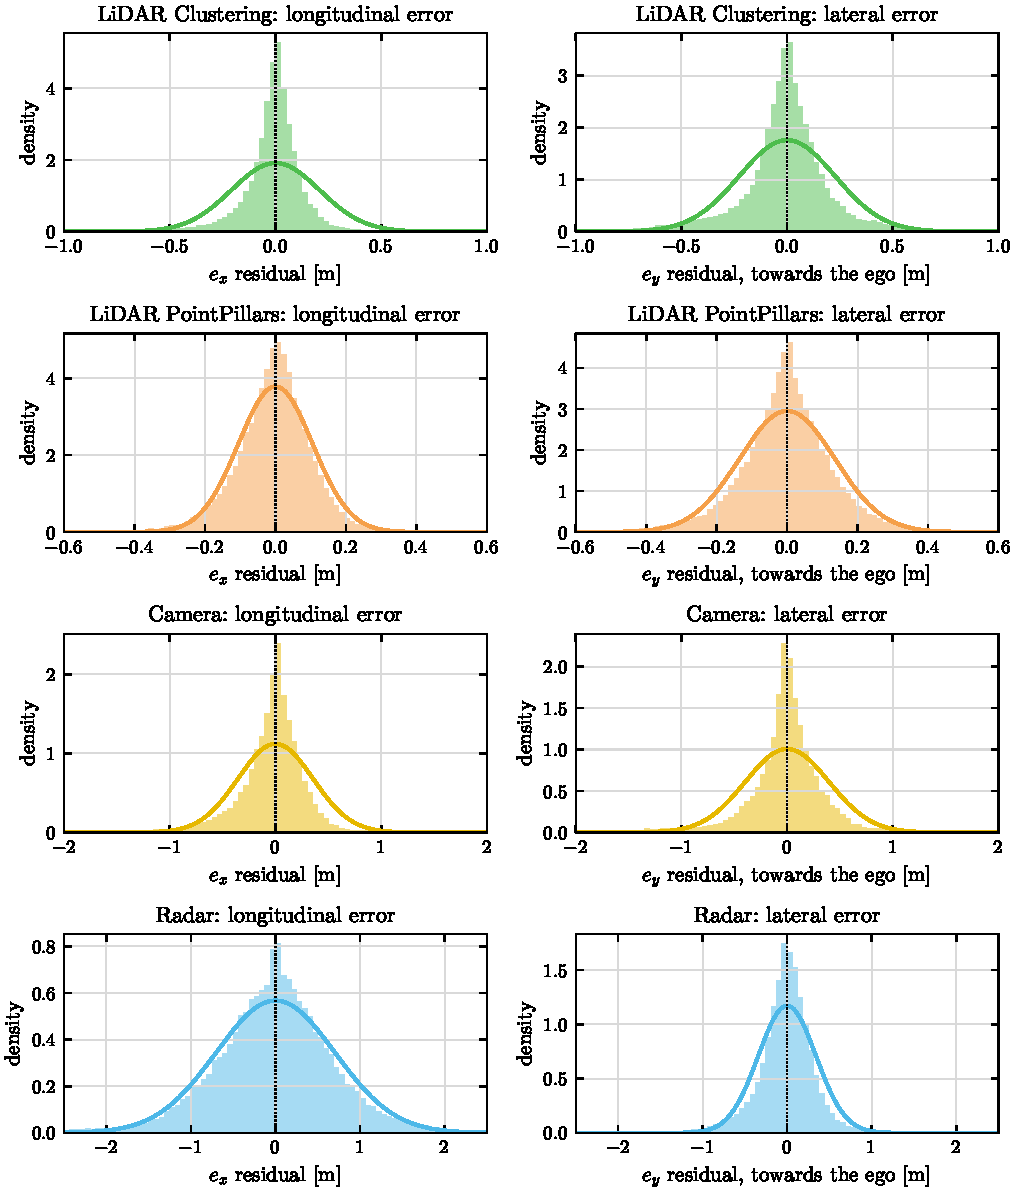
\includegraphics[width=\textwidth]{figures/ch4/gauss_std_all_sessions.pdf}
    \caption{Distributions of the residual errors of all the sessions and fitted Gaussian
    distributions.}
    \label{fig:gauss_all}
\end{figure}
